\Chapter{TradeMe}
A TradeMe egy olyan szimulációs szoftver, mely bemutatja, hogy a részvényekkel történő kereskedés lehetséges, kezdőknek adhat iránymutatást milyen feltételek mellett vásárol a program, és a megszerzett tudást átültethetik a gyakorlatba. A cél, hogy olcsón tudjon vásárolni, és később többszörös áron el tudja adni a tulajdonrészét, viszont ez nem ennyire egyszerű, a piacot sok faktor befolyásolja. A program ezeket a nehézségeket hivatott kiküszöbölni a technikai analízis eszközeit felhasználva. A szimulációhoz a limitációk miatt csak NASDAQ alá tartozó, amerikai vállalatok adatai tölthetők le.

\Section{Adatkinyerés}
A különböző tickerekhez tartozó adatok kinyerése nem egyszerű feladat, hiszen a tőzsde világában ezek az adatsorok kincset érnek. Nagyon sok szolgáltató az adatbázisát kisebb-nagyobb összegekért árulja, vagy valamilyen korlátozáshoz köti a letöltést, ezért az egyik fő feladatom, hogy olyan adatbázishoz férjek hozzá, mely ingyenes, illetve egy API-n keresztül lehetővé teszi a letöltést. Ez azért fontos, mert programozói eszközökkel könnyedén automatizálható ez a folyamat, illetve szükséges is, hogy az alrendszerek közötti egységességet biztosítani tudjam. Több lehetőséget is számításba vettem, viszont később vagy fizetőssé tették a szolgáltatást, vagy nem lett volna egyszerű a letöltési folyamat.

\subsection{Szoftveres támogatás}

Ahhoz, hogy az Alpha Vantage oldalról le tudjak tölteni adatokat, szükség van egy API kulcsra, amit a weboldalon egy egyszerű regisztrációt követően ki is küldenek. Ezután már csak annyi dolgom van hátra, hogy megfogalmazzam a lekérdezést, melyre az \nameref{alphavantage} alfejezetben bővebben kitértem.

Java nyelven készült egy kiegészítő program, amely elvégzi a megfelelő lekérdezések meghívását, letölti a 24 darab szeletet, ezeket összefűzi, majd a weboldal részéhez hozzácsatolja. Erre azért volt szükség, mert egy-egy részvény adatainak a letöltése több percet vehet igénybe, s ezzel a megoldással a háttérben futtatható a letöltés, míg a weboldalon elemezzük a részvényeket. Mivel az Alpha Vantage oldalon az ingyenes tagság korlátozásokkal jár, mégpedig azzal, hogy öt hívás lehetséges percenként, illetve egy nap maximum 500, ezért a programban szükséges rögzíteni mikor történtek a kérések. Ezt egy egyszerű listával oldottam meg, aminek \codeword{long} típusú elemei vannak. Minden letöltés után lementem az aktuális időt, s hogyha a lista mérete elérte az ötöt, akkor megnézem, hogy a legrégebbi bejegyzés óta eltelt-e 60 másodperc. Amennyiben igen, akkor a listát eltolom balra eggyel, egyéb esetben várakozik a program.

Egy lekérdezés implementációja az alábbi formában látható.

\begin{java}
String url = "https://www.alphavantage.co/query?function=" +
    "TIME_SERIES_INTRADAY_EXTENDED&symbol=" + symbol +
    "&interval=1min&slice=" + date +
    "&apikey=" + apikey;
URL website = new URL(url);
ReadableByteChannel rbc = Channels.newChannel(
    website.openStream());
FileOutputStream fstream = new FileOutputStream(
    dlDir.getAbsolutePath() + "\\" +
    symbol + "-" + date + ".csv");
fstream.getChannel().transferFrom(rbc, 0, Long.MAX_VALUE);
fstream.close();
\end{java}
Létrehozok egy url változót, ami a lekérdezést tartalmazza. A változóban három dinamikus rész szerepel: a symbol, a date, és az apikey (bővebben a \ref{alphavantage} fejezetben). Majd egy csatornát hozok létre a weboldal és a programkód között. Ezt a csatornát megkapja a FileOutputStream, amely ki tudja végül írni a lemezre a webszervertől kapott adatokat. Egy \codeword{for} ciklussal végig iterálok két év hónapjain, s így kapok 24 darab csv fájlt, amely további feldolgozásra szorul.

A második lépésben a program beolvassa egyesével a fájlokat, majd egy csv fájlba kimenti az összesnek a tartalmát. Mivel minden fájl tartalmazott fejléc részt, ezt kivágom belőlük és egy fejléc részt rögzítek a fájl első sorában.

A harmadik és utolsó lépésben a program elmozgatja abba a mappába az összefűzött állományt, amiből a weboldal alapértelmezetten kiolvassa őket, illetve az ideiglenes fájlokat törli a lemezről.

\Section{Részvény adatok feldolgozása}
A weboldal számára előkészített részvény adatokat valamilyen struktúrába szükséges rendezni, hogy később fel lehessen használni az adatokat. A részvény adatokat a program a \textbf{stocks} mappából olvassa ki a következő módon.
\begin{javascript}
$(data).find("td > a").each(function () {
    let file = $(this).attr("href").substr(1);
    file = file.substr(file.indexOf("/") + 1, file.lastIndexOf("/") -
    file.indexOf("/") - 1);

    if (file == ".." || file == "")
        return;

    tickers.push(file);
    $("#stocks").append("<option>" + file + "</option>");
});
\end{javascript}

\noindent A beolvasott sorokon végig iterál a program és kiválogatja belőle a dátumokat és a hozzájuk tartozó záróárakat. Mivel az adatsorok több százezer bejegyzést is tartalmazhatnak, ezért úgy döntöttem, hogy külön tömbben tárolom a dátumokat és a záróárakat. Ez azért is fontos, mert később szükség lesz a grafikon készítésénél a dátumra külön, hiszen hozzá kell rendelni minden adatot a megfelelő időponthoz.

\Section{Statisztikák számítása}
A kereskedésnél a technikai elemző stílust választottam, amely indikátorokat is vizsgál, és az ismereteit összegezve hoz döntést a részvényeiről. Az én szoftverem is az indikátorokat használja a vásárlás/eladás döntés meghozatalához, viszont az elkészítésüknél több problémába is ütköztem.

A statisztikai számításokban megjelenik a periódus paraméter, mely meghatározza hány adatból kalkuláljon az algoritmus egyet. Ha egyszerűen két \codeword{for} ciklust készítünk hozzá nem törődve az iránnyal, hamis eredményt kaphatunk.
\begin{figure}[ht]
\centering
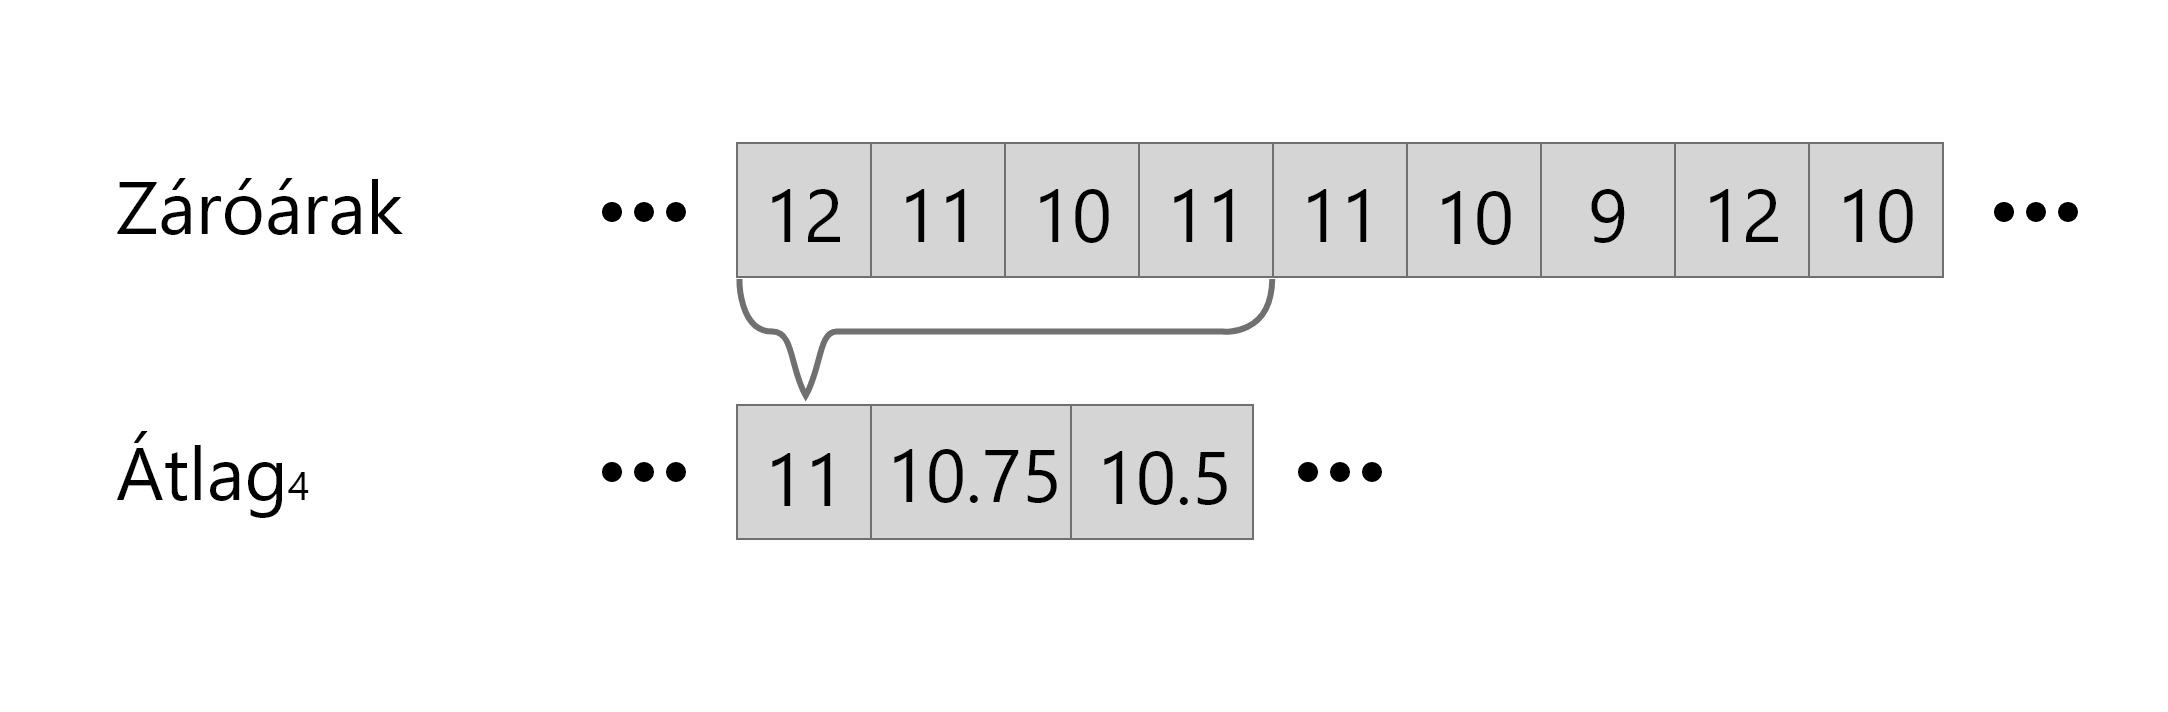
\includegraphics[scale=0.18]{images/stat.png}
\caption{Átlag számítása 4-es periódus értékkel előrefelé.}
\label{fig:stat}
\end{figure}

\noindent Hogyha előrefelé haladunk a ciklussal, akkor azt tapasztaljuk a futtatásnál, hogy hitetetlen összegeket tud gyűjteni a program, és ez azért van, mert jövőbeni adatokat veszünk figyelembe. Ha történik egy hirtelen irányváltás a részvény árában, akkor az indikátorok ezt mindig később fogják jelezni, ahogyan \aref{fig:trend}-es ábrán látható. Ezért, ha előrefelé haladunk, akkor ezeket a jelzéseket is előrébb hozzuk, ami életszerűtlen. A szimulációs környezet miatt, illetve a futási idő javítása érdekében a statisztikák előre elkészülnek, viszont a való életben úgy frissülnek az indikátorok, ahogyan érkeznek az adatok.

Második probléma, ami előbukkant a tesztelések során, az a futási idő. Összesen 8 darab indikátort számít ki a program, amelyből a legegyszerűbbet emelem ki, az SMA-t. Az SMA-nak a számításához két \codeword{for} ciklus szükséges, ami összesen $((\text{adatmennyiség} - \text{periódus} - 1) * \text{periódus})$ számítást végez el, s az alábbi módon implementáltam.
\begin{javascript}
function WcalcSMA(arr, end, period) {
    let tmp = [];
    for (let point = 0; point < end; point++) {
        let sum = 0;

        if (point < period - 1) {
            tmp.push(0);
        } else {
            for (let i = point; i > point - period; i--) {
                sum += arr[i];
            }
            tmp.push(parseFloat((sum / period).toFixed(6)));
        }
    }
    return tmp;
}
\end{javascript}
Ez nem nagy feladat a processzornak, viszont érdemes megfontolni az iteráció helyét. Az árfolyamok nagysága miatt érdemesebb a ciklust az adott statisztikát számító függvénybe helyezni, mert így egy függvényhívással elvégezhető egy indikátor számítása. Ezzel szemben, ha egy ciklusban hívom meg az összes függvényt, amik egy pontot számítanak ki, akkor a hatalmas mennyiségű függvényhívás lelassíthatja a futást.

A statisztikákat külön szálon számítom ki, hogy a felhasználó számára ne okozzon negatív élményt, ne fagyjon le addig a grafikus felület kezelője. Egy statisztikának a kiszámítása az alábbiak szerint néz ki.
\begin{javascript}
function createWorker(i) {
    return new Promise(function (resolve) {
        let w = new Worker('/js/worker.js');

        w.postMessage(i);
        w.onmessage = function (event) {
            w.terminate();
            resolve(event.data);
        };
    });
}

message = {type: "RSI", data: [closePrices, endPoint, 14]};
promises.push(createWorker(message));
\end{javascript}
Létrehozok egy új Workert, aminek egy üzenetet kell küldeni, amit az ő feldolgozója értelmezni tud. Meg kell adni a típusát az indikátornak, illetve a paraméterlistáját, ez esetben a záróárak tömbjét, a feldolgozandó elemek mennyiségét, illetve az indikátor periódusát. Ez alapján meghívja a megfelelő függvényt, ami egy tömbben összesíti az eredményeket, és ezt visszaküldi a csatornán (\ref{fig:jsww}-es ábrán szemléltetve). A visszaérkező üzenetek olyan sorrendben jönnek, mint amilyen sorrendben küldtem őket, ezért nem kell ügyelni az esetleges keveredésekre.

\Section{A kereskedés menete}
A weboldal az alábbi felülettel fogad megnyitáskor.
\begin{figure}[ht]
\centering
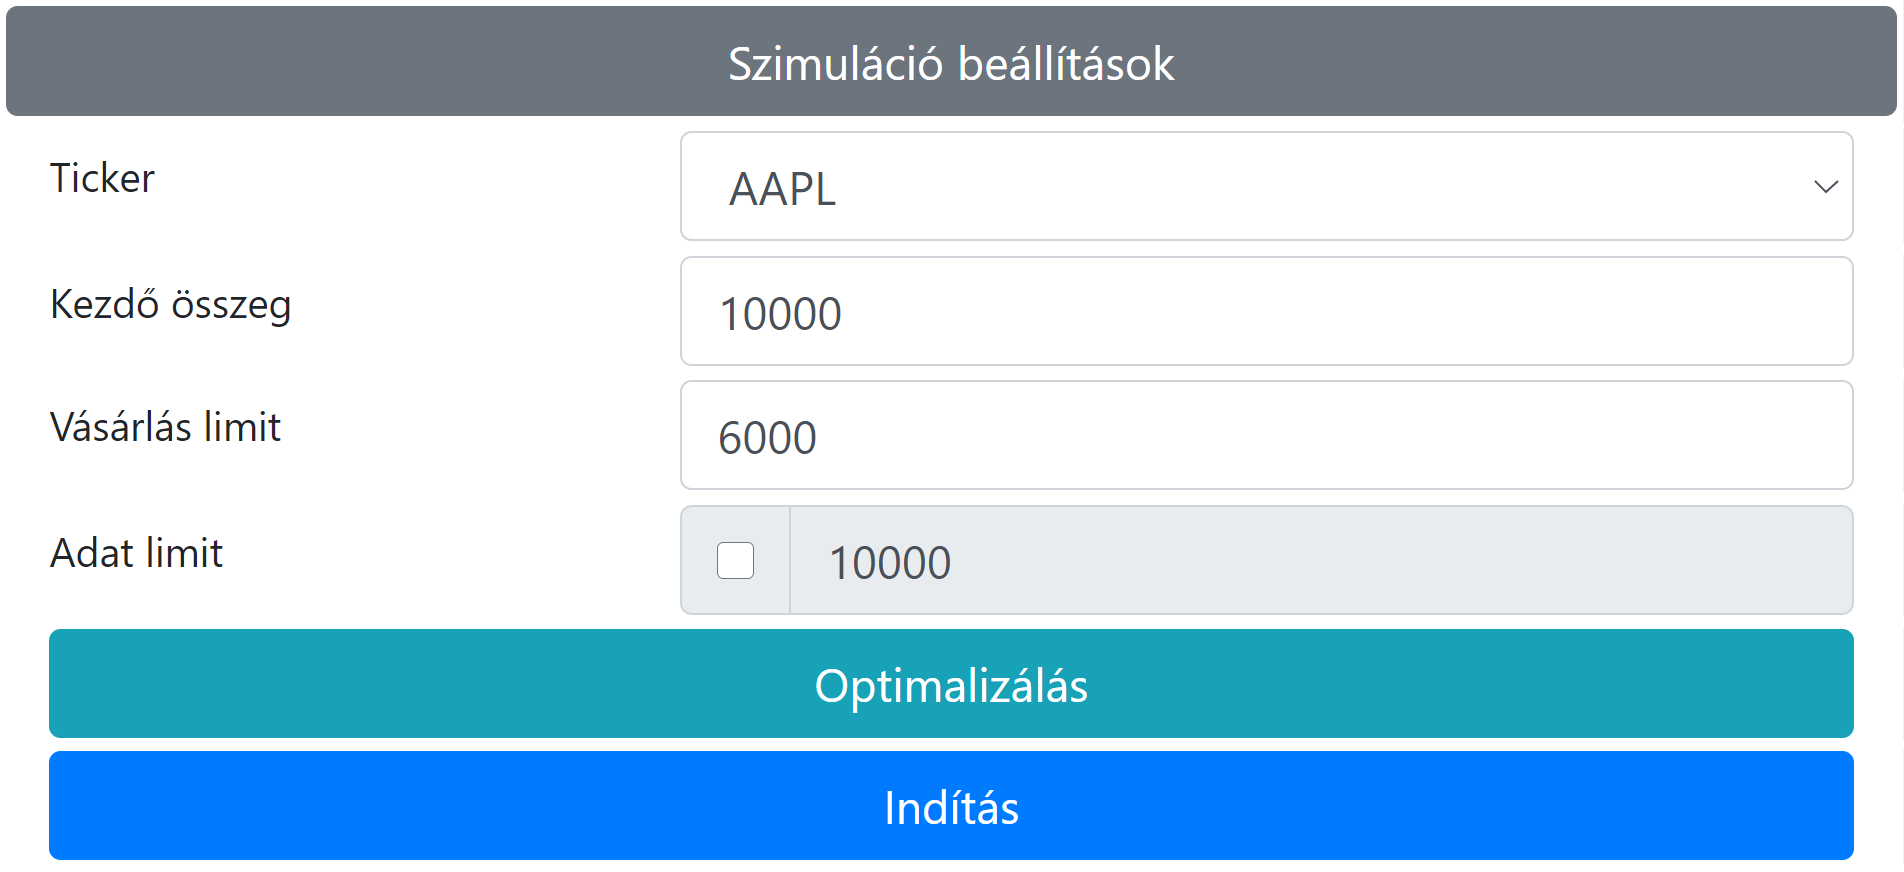
\includegraphics[width=\textwidth]{images/website.png}
\caption{A webes felület nyitóoldala.}
\label{fig:website}
\end{figure}
A program automatikusan felismeri a helyesen elhelyezett részvényeket és betölti, s egy legördülő menüből választhat a felhasználó közülük. A kezdő összeg mezővel beállítható, hogy mennyi pénzzel kezdjen el gazdálkodni a program. Alapértelmezettként 10 000\$-t adtam meg, hiszen például az Interactive Brokers cég minimális számlanyitási összegét így állapították meg, azonban eltérő lehet cégenként \cite{solyomi2017}. A vásárlási limit beállítás arra való, hogy korlátozza az egy tranzakcióra eső elkölthető pénz mennyiségét. Létezik egy joker lehetőség, ha $(-1)$-et ad meg a használó, akkor mindig elkölti az összes pénzt részvényekre. Az adat limit paraméter leginkább arra használható, hogy leválasszon a program $x$ darab záróárat, így kis adatbázissal gyorsabb lekérdezést, illetve gyorsabb grafikont lehet elérni.

\subsection{Vásárlási limit beállítása}
A vásárlási limit egy olyan beállítás, ami nagyban befolyásolhatja a program vásárlási szokásait. Meghatározza, hogy mekkora profittal zárja a kereskedést, hogy mennyi tranzakciót végez. Ezt az adatot érdemes valamilyen módszerrel az optimumhoz közelíteni, hiszen ekkor keres a legtöbbet vele a program. Az alábbi ábrán látható, hogy a különböző részvények a 10 000\$-os induló összegüktől mennyivel térnek el a szimuláció végére.
\begin{figure}[ht]
\centering
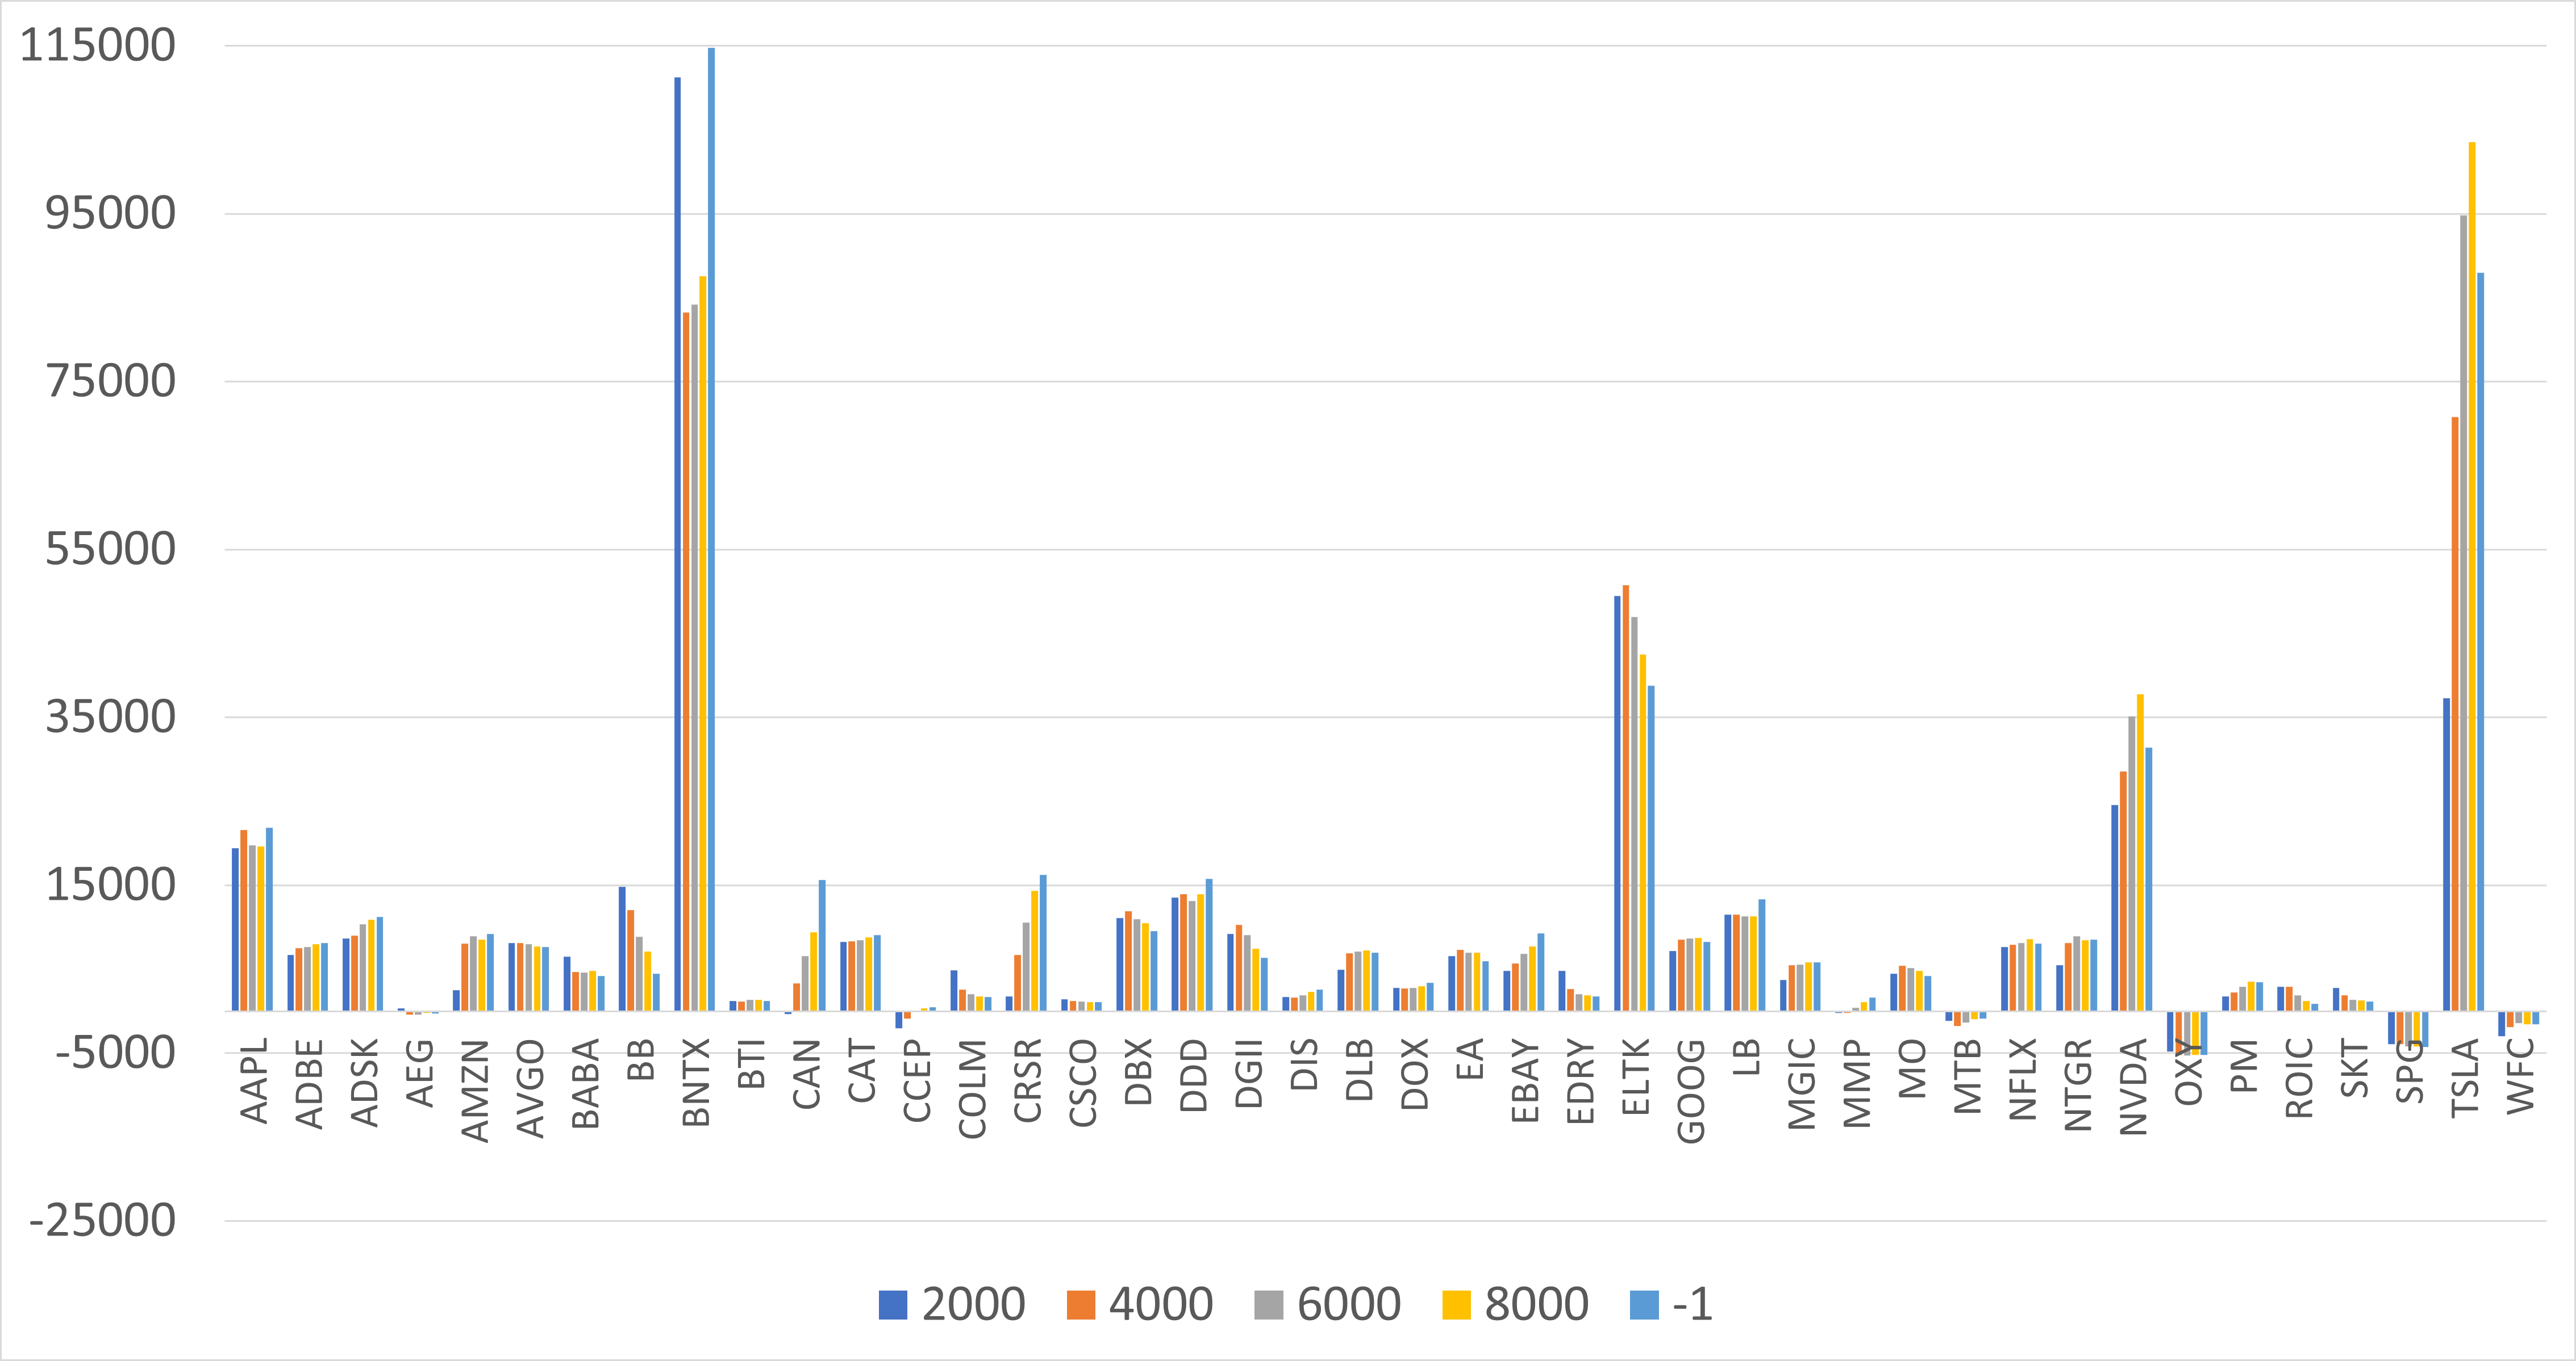
\includegraphics[scale=0.42]{images/limitdiag.png}
\caption{A részvények profitjai vásárlási limit függvényében.}
\label{fig:limitdiag}
\end{figure}
Ha megnézzük például a NFLX, azaz a Netflix eredményeit, akkor azt láthatjuk, hogy egészen közel vannak az eredményei egymáshoz, a maximumát a \mbox{8 000}-es limitnél éri el (\ref{fig:NFLX}-es ábra).
\begin{figure}[ht]
\centering
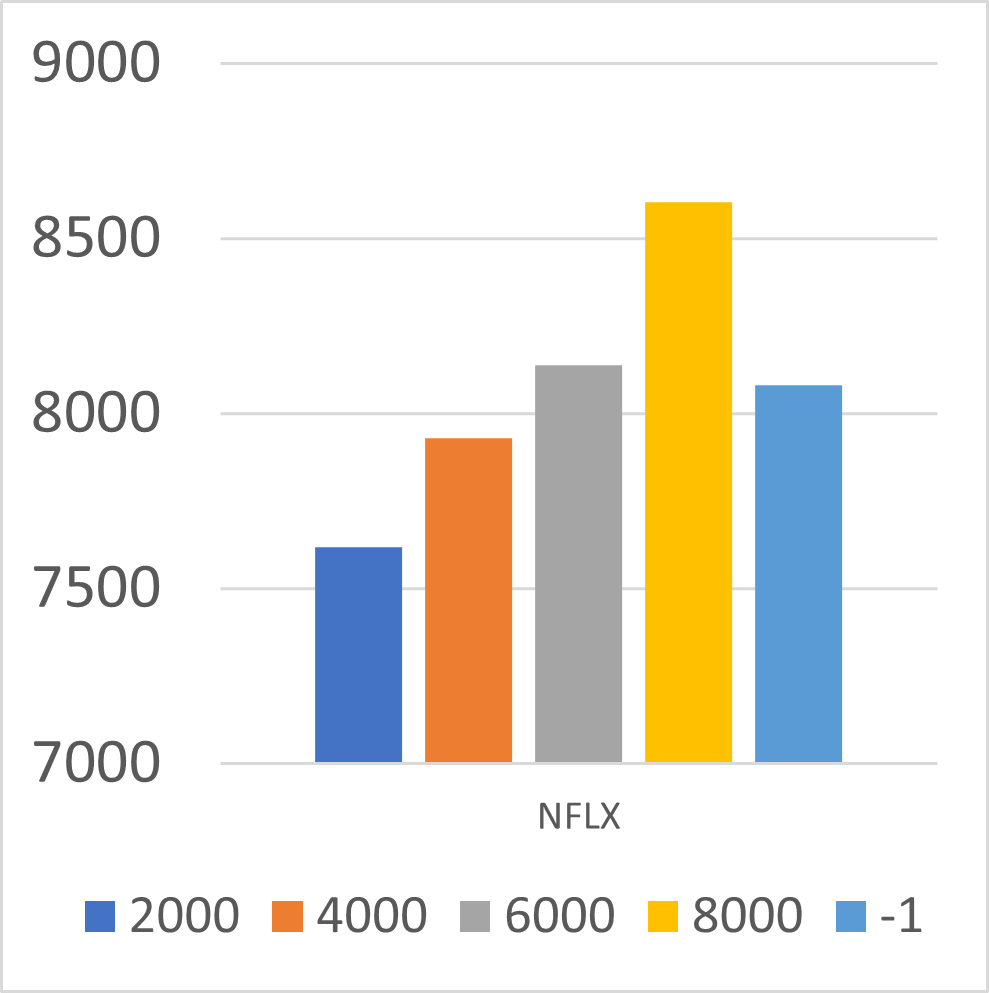
\includegraphics[scale=0.7]{images/NFLX.png}
\caption{A Netflix profitja különböző vásárlási limitekkel.}
\label{fig:NFLX}
\end{figure}
Mindegyik beállításnál profitot termelt, azonban vannak olyan részvények is, amik a limit növelésével a profit, illetve olyanok is, amik a veszteség irányába változnak. Összességében az mondható el, hogy a profitok összege a maximumát a $(-1)$ esetben éri el, azaz amikor az összes pénzét elkölti a program egy-egy vásárlásnál (\ref{fig:limitdiag}-es ábra).

\subsection{Kereskedési feltételek}
A szakdolgozatom egyik legnehezebb része a vásárlási, illetve az eladási feltételek meghatározása volt. Az indikátorok megléte még önmagában nem garantálja a sikert, meg kell mondani az algoritmusnak, hogy melyek azok az alakzatok, amelyek bebiztosítják a sikert. Összesen 5 féle alakzatot definiáltam a programban vásárlási és eladási célra, amelyekek súlyozását utána a genetikus algoritmus segítségével optimalizáltam. A három legmeghatározóbb alakzat között szerepel az MACD növekedése és csökkenése. Ekkor 20 periódussal nézem visszafelé az adatokat, és hogyha nem tapasztalok egymás után kétszer csökkenést, akkor a függvény irányát felfelé haladónak tekintem. Ha teljesül a növekedés feltétele, vagy az MACD éppen 0 fölötti értéken szerepel, akkor a vásárlást eldöntő változóhoz hozzáadom a súlyozási értékét az alábbiak szerint.
\begin{javascript}
if (macdArr[i] > 0 || macdRising(i)) {
    decision.buy += mutant[4];
}
\end{javascript}
A genetikus algoritmus ezt a jelzést 9.15 pontra értékelte a maximum 10-ből.

A következő mutató, amit szeretnék megemlíteni az RSI-vel van összefüggésben. Az RSI-nél két határ szoktak nézni, a jelzésnél a 30-as határt vizsgálom éppen, a következő módon.
\begin{javascript}
if (rsiArr[i] < 30) {
    decision.buy += mutant[6];
}
\end{javascript}
Ha az RSI 30 alá menne, akkor alulértékelt a részvény, tehát érdemes megfontolni a vásárlást. Az optimalizáció során 6.35 pontot kapott, azaz a második leghasznosabb indikátor a gyűjteményből.

A harmadik legtöbb pontot kapott indikátor már az eladási jelzések közé tartozik. Azt vizsgálja, hogy az MACD negatív szám-e, vagy csökkenést mutat-e az MACD. Ez az alakzat az elsőnek a megfordításából adódik, azaz a következőképp írható le.
\begin{javascript}
if (macdArr[i] < 0 || !macdRising(i)) {
    decision.sell += mutant[5];
}
\end{javascript}

\noindent A következő felsorolásban a többi általam implementált jelzést foglalom össze röviden.
\begin{itemize}
  \item Amikor a $\text{SMA}_{200}$ felülről metszi az $\text{SMA}_{50}$-et, akkor aranykeresztről beszélünk, ellentétes esetben halálkeresztről, előbbi a vásárlási, utóbbi az eladást jelző alakzat.
  \item Ha az MACD keresztezi a szignálját felülről, akkor vásárlási, egyébként eladási jelzőként szolgál.
  \item Az RSI-nél egy szigorúbb feltételt is szerepeltettem a 20-as és a 80-as határokra, hogy erősítsem az indikátor jelzéseit nagyobb kilengés esetén.
\end{itemize}
Ezeket az adatokat a \textbf{decision} objektumban összegzem. Ha a \textbf{sell}, vagy a \textbf{buy} paramétere nagyobb lesz mint 10, akkor az annak megfelelő függvényt meghívom. Ha végig fut a program az összes értéken, akkor visszatérek a végösszeggel, s ha normál módban van a program, akkor kiírja a végeredményt. Ha profitot termelt a program, akkor zöld színnel, ha bukott, akkor piros színnel jelenítem meg a végösszeget. A végösszeg nem csak a profitot tartalmazza, hanem a kezdőösszeget is. Az alábbi képen látható, hogyan néz ki egy végállapot.
\begin{figure}[ht]
\centering

\includegraphics[width=\textwidth]{images/website_results.png}
\caption{Pénztárca tartalma, illetve a tranzakciók száma a szimuláció végén.}
\label{fig:website_results}
\end{figure}
\begin{figure}[ht]
\centering
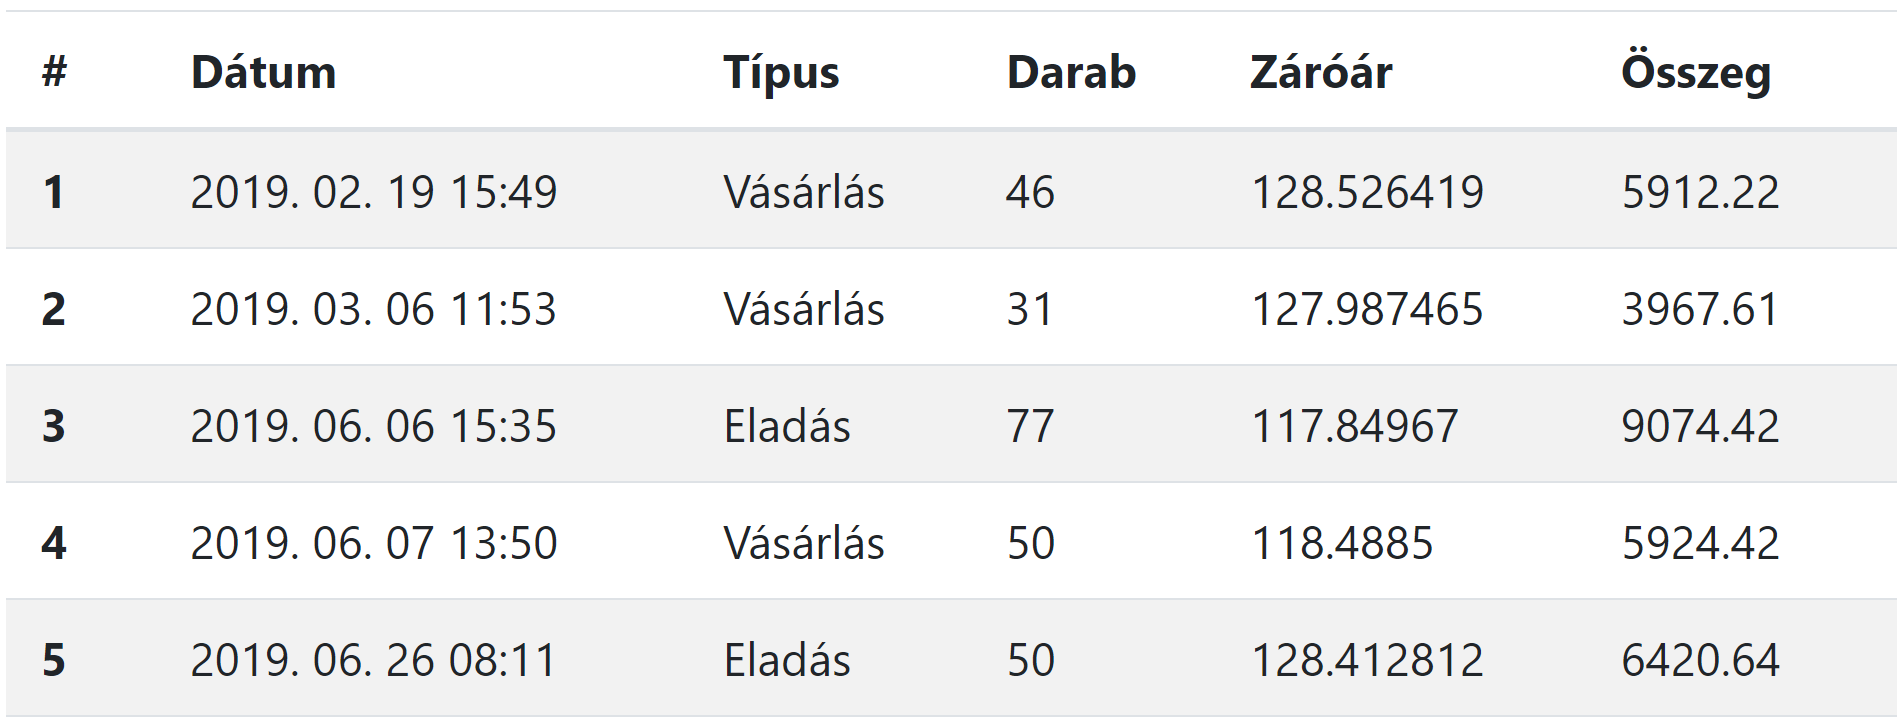
\includegraphics[width=\textwidth]{images/website_transactions.png}
\caption{A szimuláció végén generálódó tranzakciós lista.}
\label{fig:website_transactions}
\end{figure}
A tranzakciós tájékoztató egy interaktív elem, gombnyomásra lenyílik, s kiírja az összes tranzakciót, ami történt (\ref{fig:website_transactions}. ábra).
Látható erről az öt adatról is, hogy a vásárlási limitet 6 000-re állítottam be, hiszen az első és negyedik vásárlás nem lépte túl ezt a mértéket. Továbbá, ha megnézzük az adatokat, akkor azt mondhatjuk, hogy az első eladáskor 805\$ deficit keletkezett, azonban a következő tranzakció pároson már részvényenként 10\$ hozamot ért el a program. A következő kódrészlet írja le azt, ahogyan megjelenik a tranzakciós lista.
\begin{javascript}
$("#transactionsTable").append(
    '<tr><th scope="row">' + (counter++) + '</th>' +
    '<td>' + formatDate(new Date(tr.date)) +
    '<td>' + ((tr.type == "buy") ? 'Vasarlas' : 'Eladas') +
    '<td>' + tr.amount +
    '<td>' + parseFloat(tr.stock_price.toFixed(6)) +
    '<td>' + parseFloat((tr.stock_price * tr.amount).toFixed(6)) +
    '</tr>');
\end{javascript}

Ha tovább görgetünk a weboldalon, akkor a legalján egy grafikon található. A grafikonon megjelenítem a záróárakat, az 50, illetve 200 periódusú SMA-kat, az RSI indikátort a 30-as és 70-es határértékeivel, az MACD-t és a szignál függvényét, végezetül a vásárlási és eladási pontokat. A grafikonon megjelenő adatok ki és bekapcsolhatók a menüsor közepén található feliratokkal. Az adatok mennyisége miatt érdemes kikapcsolni addig bizonyos függvényeket, míg navigálunk a grafikonon, hiszen nagyon erőforrásigényes tud lenni nagy adatsorokon.
\begin{figure}[ht]
\centering
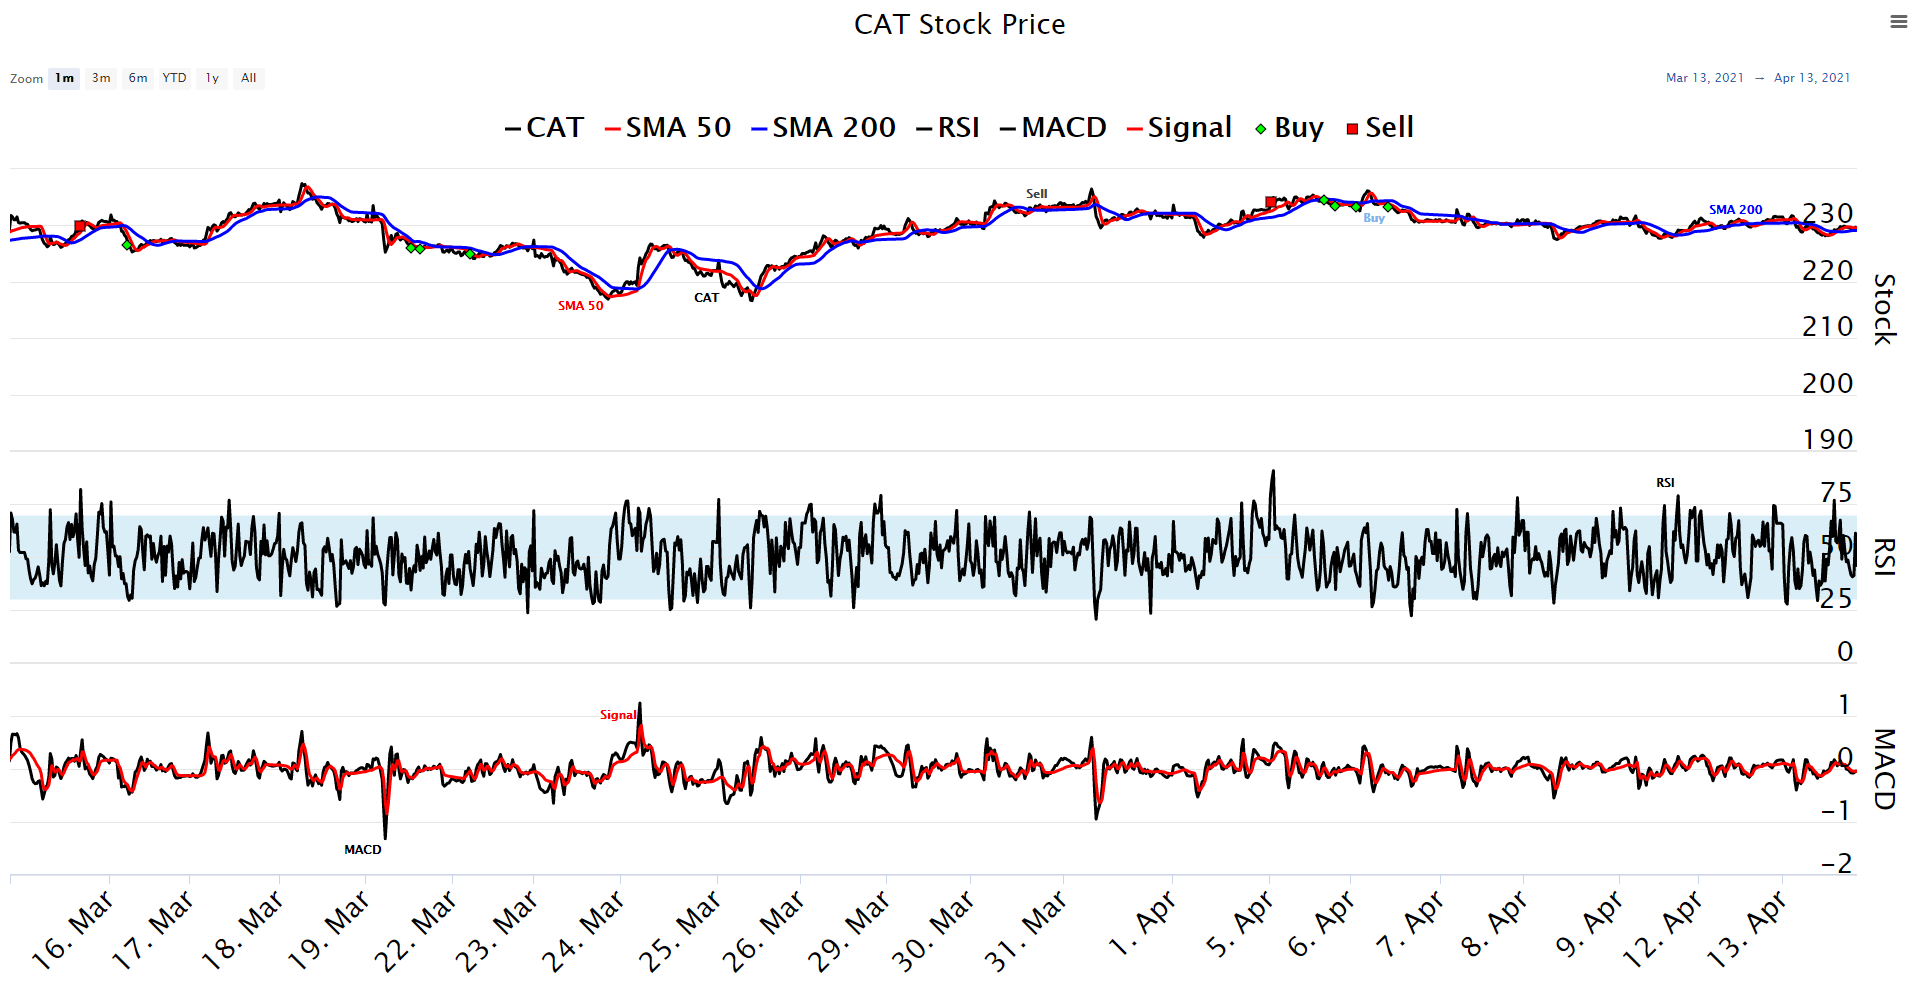
\includegraphics[width=\textwidth]{images/website_chart.png}
\caption{A szimuláció végén generálódó grafikon.}
\label{fig:website_chart}
\end{figure}
\newpage
\Section{Legjobb kromoszóma megtalálása}
A szimuláció önmagában haszontalan, hiszen az indikátorok megfelelő súlyozását ki kellene találni, vagy ha szerencsénk van egyből a legjobbat találjuk meg, azonban ennek kicsi az esélye. Ennek a kiküszöbölésére vezettem be a genetikus algoritmust, mely optimalizálja nekem a problémát.

A kezdeti populáció 10 elemű és 11 darab gént tartalmaznak, amely megegyezik a feltételek számával a kereskedésnél. Minden gén inicializálásra kerül, egy 0 és 10 közötti számot kapnak kezdeti értéknek. Ezután meghívom a \textbf{newGeneration} függvényt, mely először kiszámítja a generált populációra a fitness értékeket. A fitness értékek a következő számításon alapszanak.
\begin{javascript}
function calcFitness(start_money, end_money) {
    return end_money / start_money;
}
\end{javascript}
Miután kiszámította a fitness értékeket, megkeresem közülük a maximumot, hiszen a legjobbat nagyobb valószínűséggel szeretném megtartani. Ezért a következő szakaszban végig iterálok a populáción, és a fitness függvény alapján sokszorozom a kromoszómákat. Minél nagyobb egy kromoszóma fitness értéke, annál többször szerepel a gyűjteményben. Majd ebből a gyűjteményből véletlenszerűen kiválasztok két kromoszómát, és keresztezem őket szimmetrikusan.
\begin{javascript}
function crossover(a, b) {
    let len = a.length;
    let midpoint = Math.floor(Math.random() * len);

    let child = a.slice(0, midpoint).concat(b.slice(midpoint, len));

    return child;
}
\end{javascript}
A kapott kromoszómára még egy mutáló függvényt meghívok, ekkor lesz kész egy új eleme az új populációnak.
\begin{javascript}
function mutate(child) {
    return child.map(e =>
        Math.random() < 0.1 ? getRandomNumber() : e
    )
}
\end{javascript}
Miután meglett az új populáció, újra meghívom a függvényt, és kezdődik előről a ciklus. Mindaddig fut, amíg el nem éri a 100 iterációt úgy, hogy nem javult semennyit a fitness függvény.

A végeredményt manuálisan szükséges eltárolni a \textbf{weights.js} fájlban, viszont már alapból a legjobb fitness függvényű kromoszóma szerepel benne a letöltött adatokon vizsgálva. Amennyiben szeretnénk saját magunk elkészíteni az optimalizálást, abban az esetben ki kell választani egy részvényt, és az optimalizálást gombot megnyomni. Ekkor lefut a genetikus algoritmus, majd kiírja a fitness függvény értékét. Ezt leokézva a következő ablakban a letöltés indul el, a weboldal mappáján belül a \textbf{js} mappába szükséges menteni.

\Section{A tőke alakulása a szimuláció alatt}
A kereskedés ideje alatt érdekes információkat tudhatunk meg abból, hogyan változik a tőke összege. Nem mindegy, hogy elbukjuk az induló tőkét, és visszaszerezzük, vagy éppen egész jó profit volt végig és a végén elbuktuk az egészet. A következő grafikonokon három részvényt mutatok be: egy jól, egy közepesen, és egy rosszul teljesítő részvényt.

A jól teljesítő részvényhez a Tesla részvényét választottam. Mint látható, 10 000\$-ból 95 728\$-ig jutott el. Eleinte lefelé indult, a veszteség irányába, minimum értéke \mbox{6 480\$} volt, azonban hamar megfordult a görbe és meredeken döntötte a profitokat.
\begin{figure}[ht]
\centering
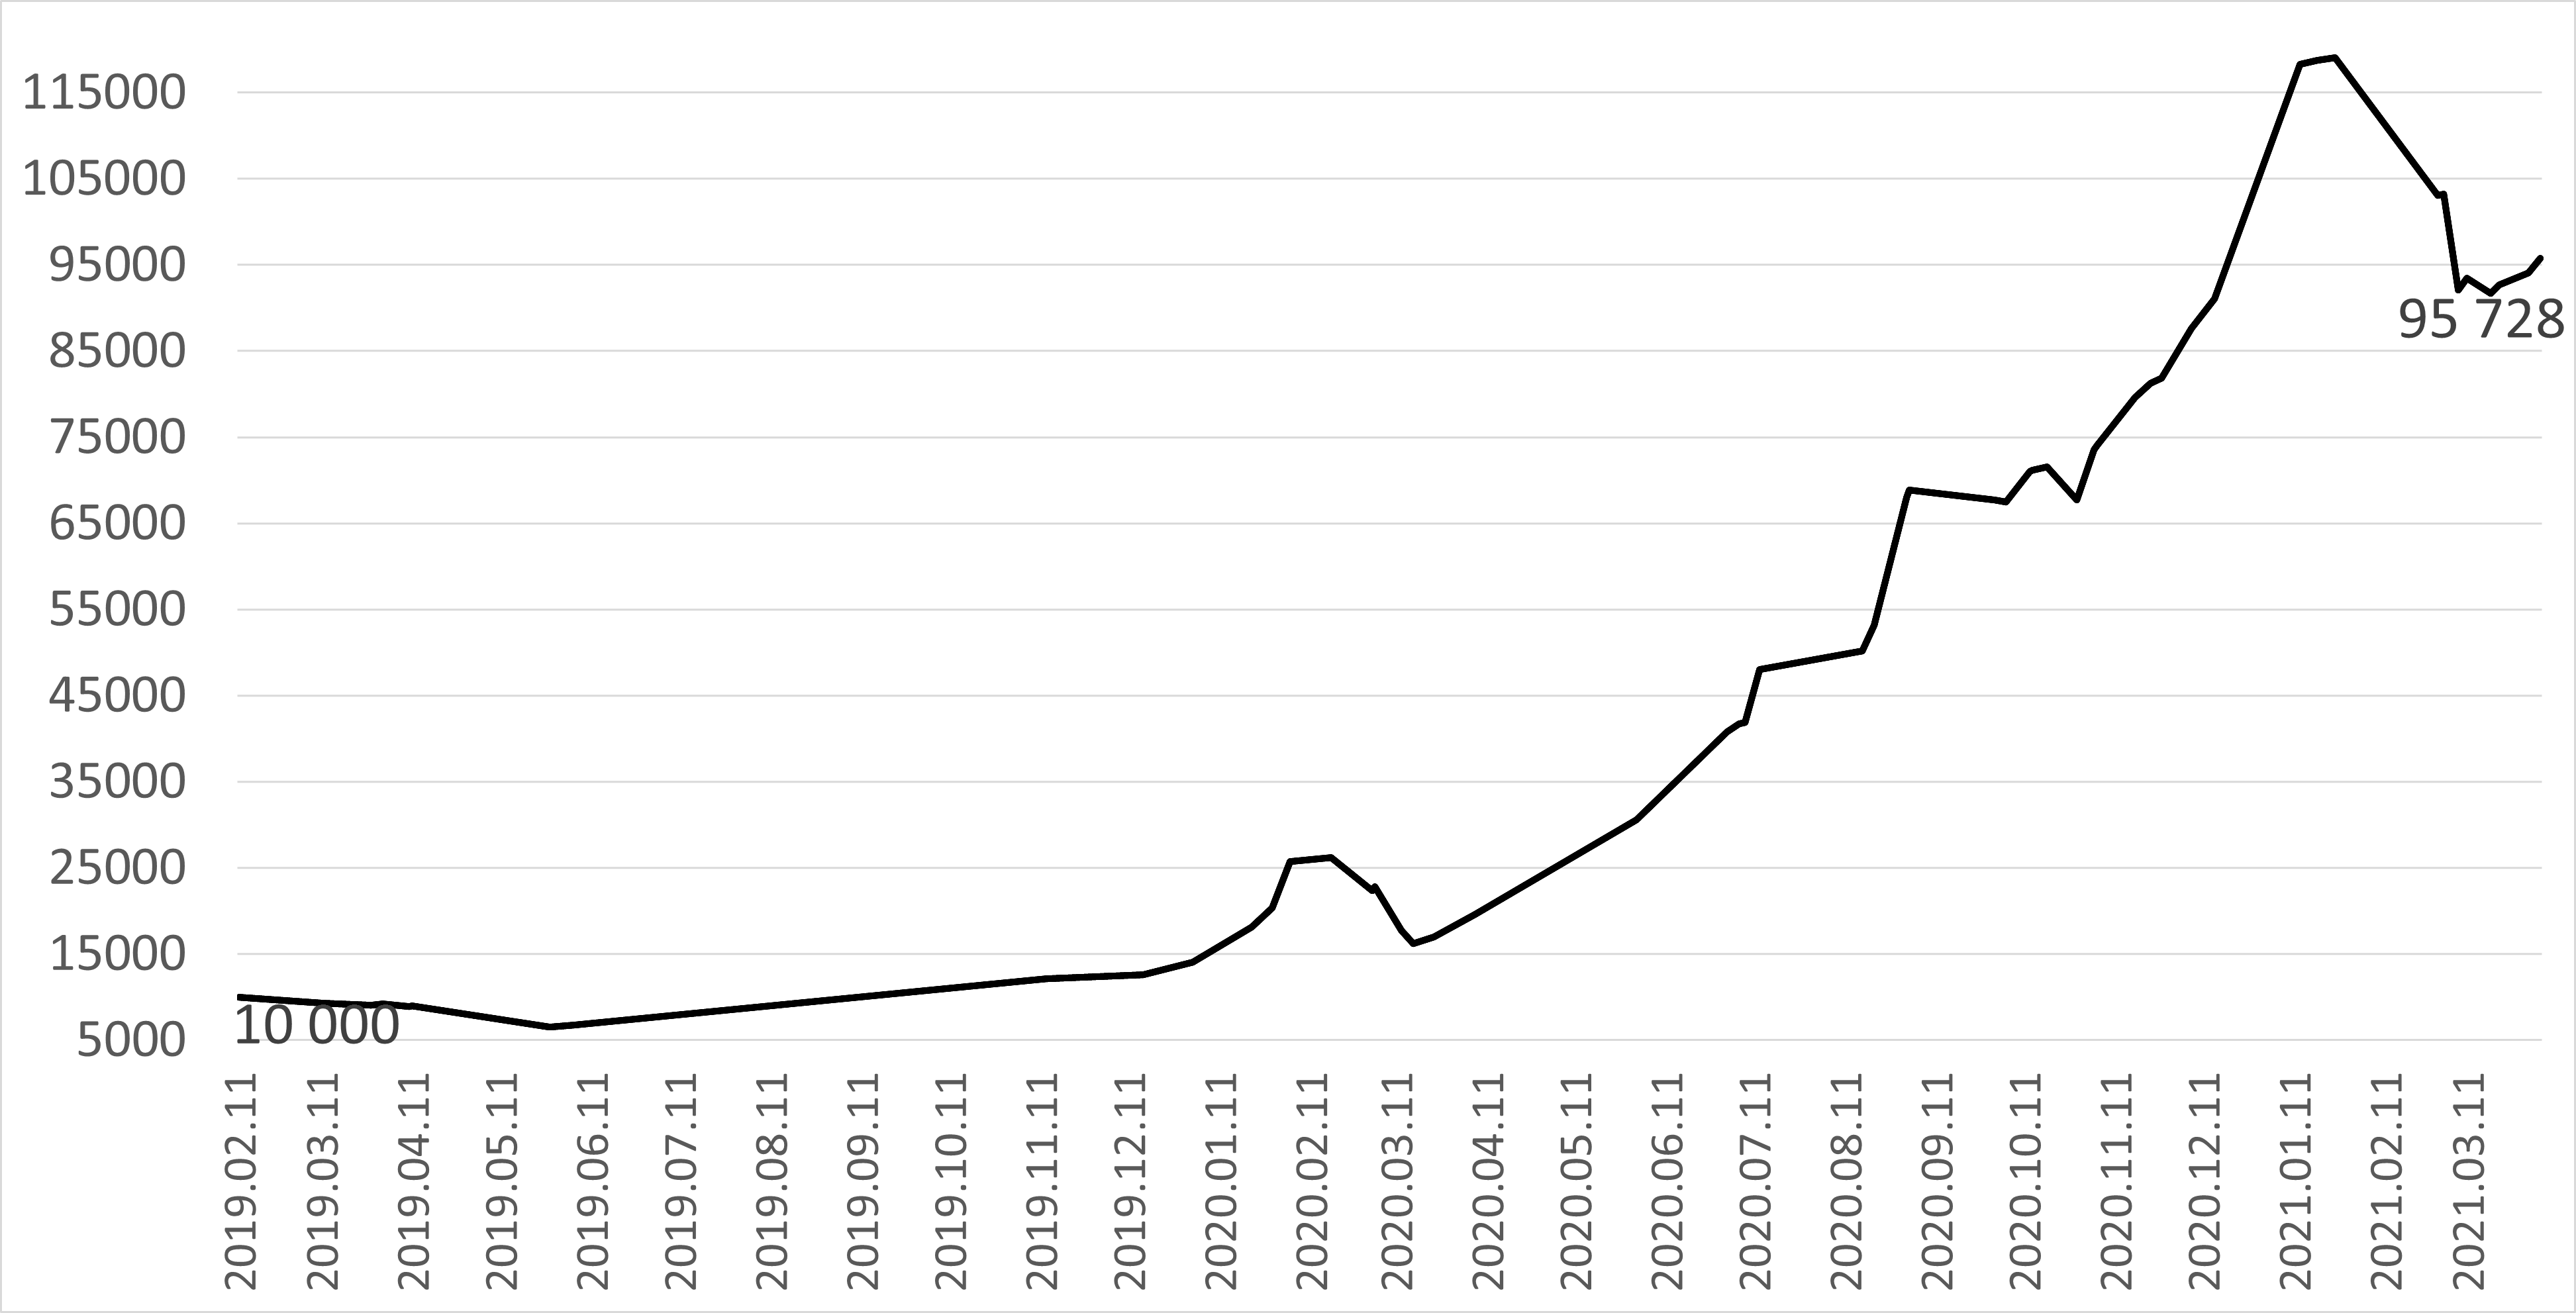
\includegraphics[scale=0.47]{images/TSLA_MONEY.png}
\caption{A tőke ingadozása a Tesla részvényén.}
\label{fig:TSLA_MONEY}
\end{figure}

A következő részvény, melyet vizsgálat alá vontam, az az Apple részvénye. 26 686\$-os végösszegével átlagosnak mondható, ha az összes részvényt tekintjük (vizsgált részvények a \ref{fig:limitdiag} ábrán). Ennél a részvénynél nem tapasztalható negatív szakasz, azaz sosem ment 10 000\$ alá.
\begin{figure}[ht]
\centering
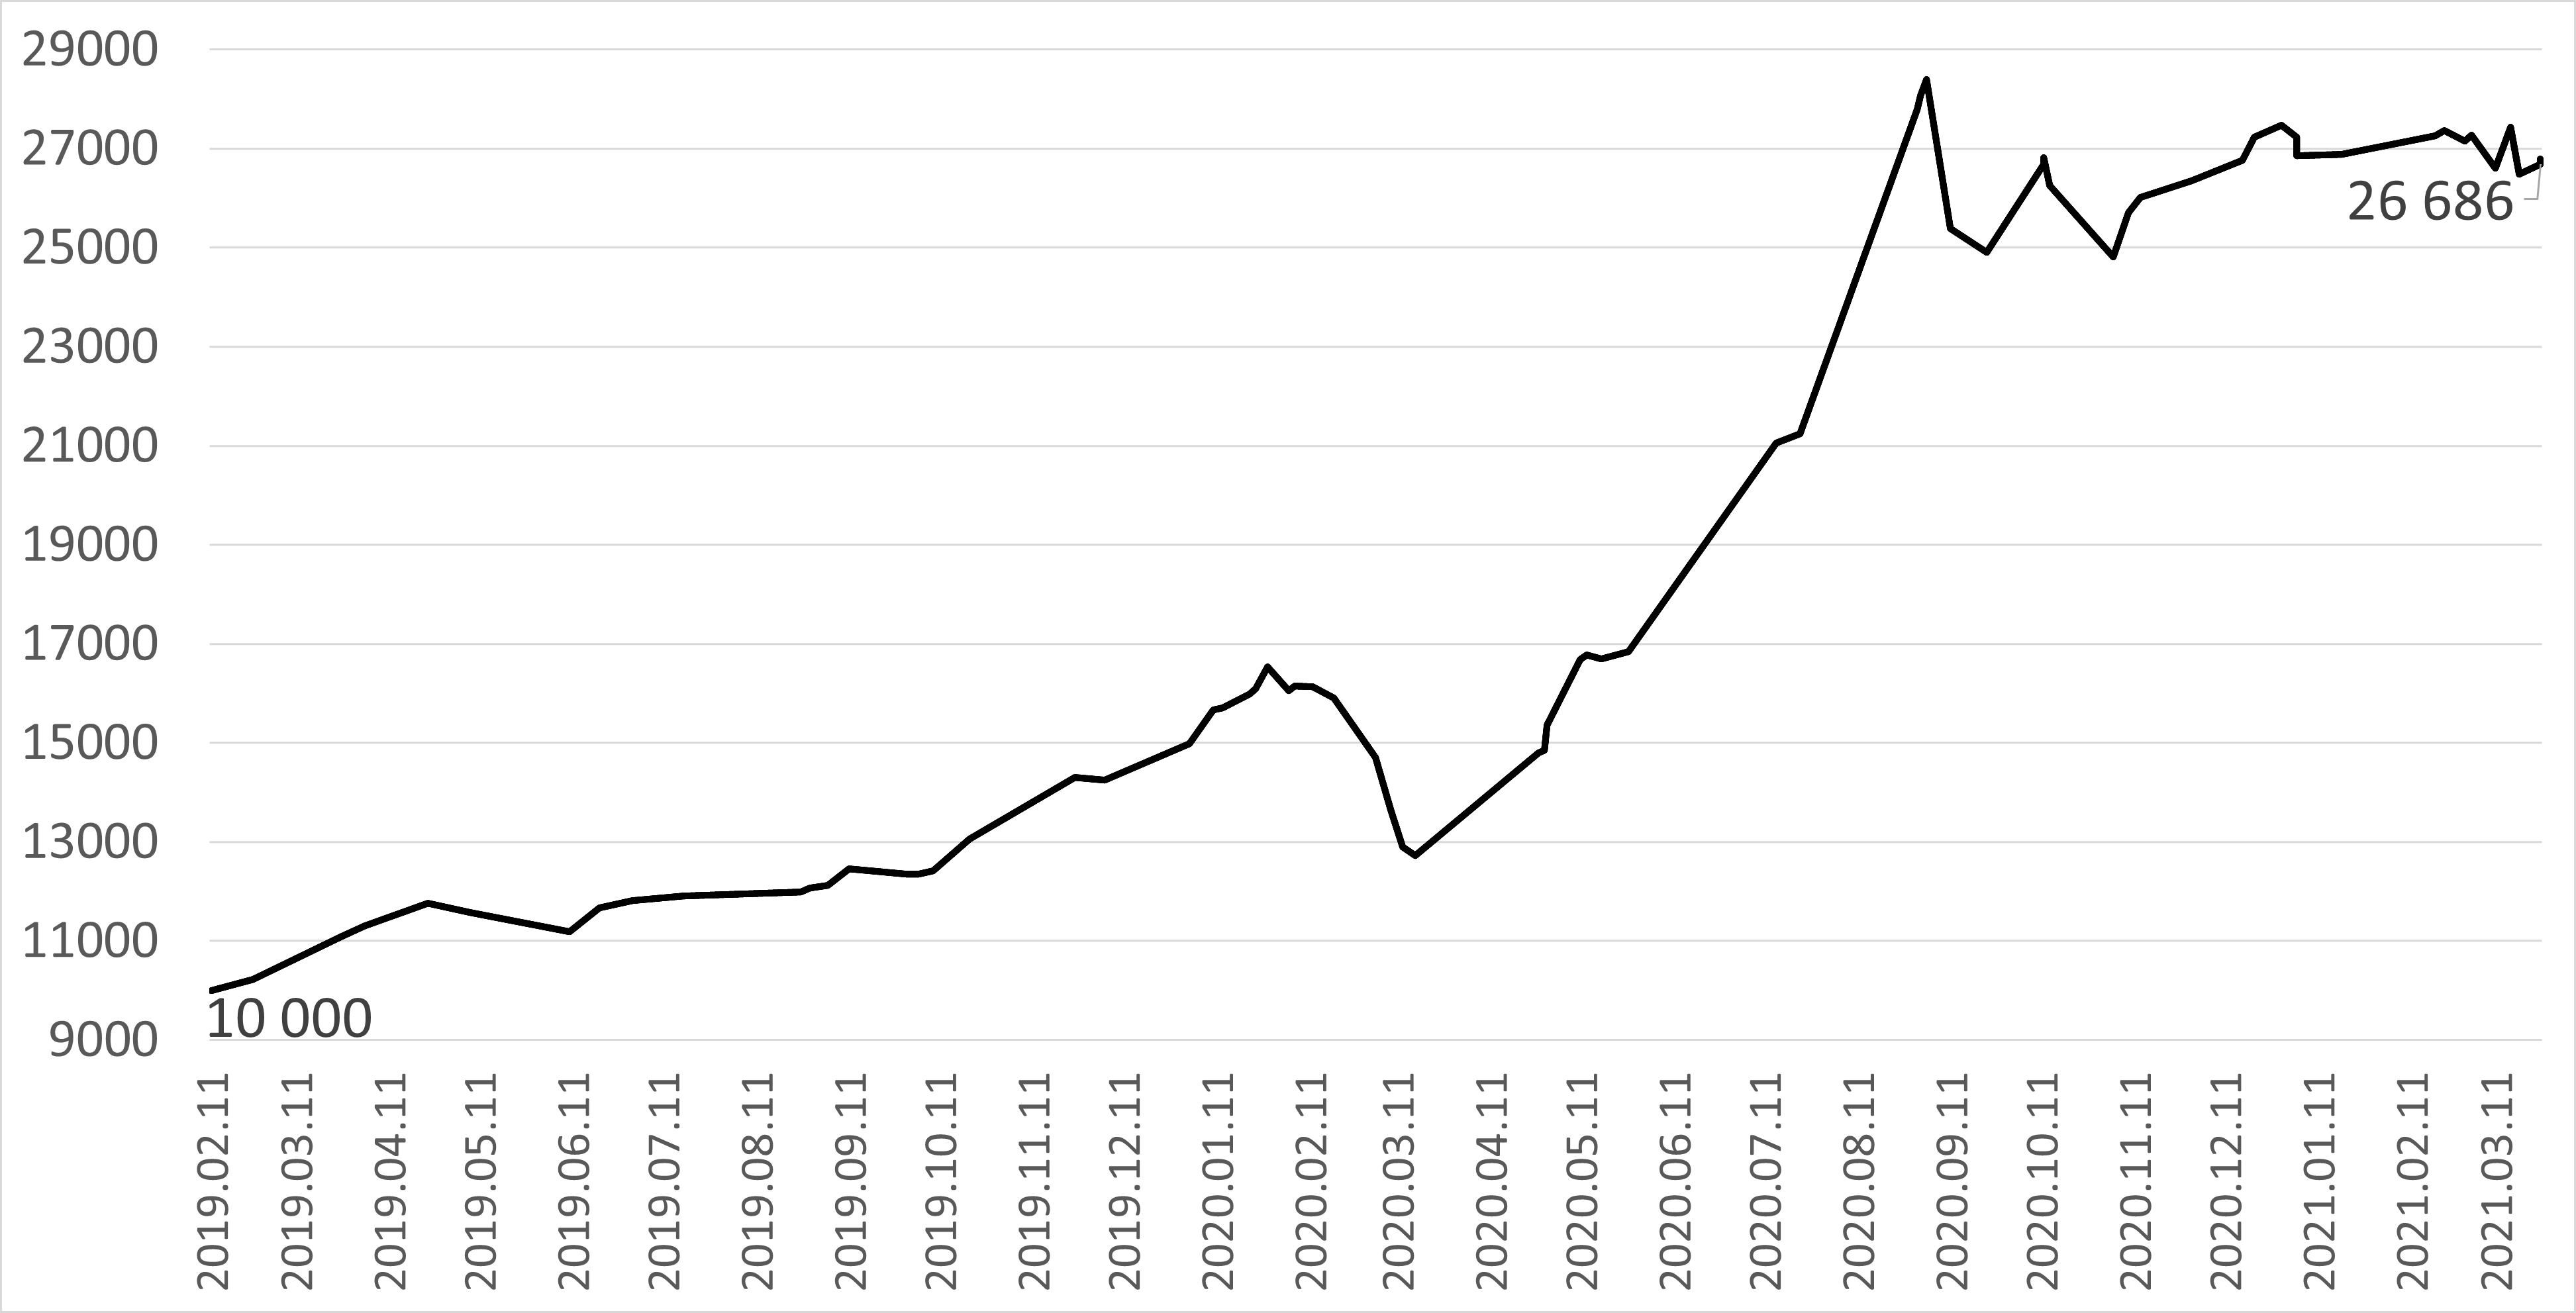
\includegraphics[scale=0.47]{images/AAPL_MONEY.png}
\caption{A tőke ingadozása az Apple részvényén.}
\label{fig:AAPL_MONEY}
\end{figure}

Az utolsó részvény a listából a rosszul teljesítő kategóriába esik, az OXY részvénye. Egy rövid felfelé ívelés után folyamatos bukás jellemzi a görbéjét. Később próbált rendeződni az tőke, elképzelhető, hogy egy év múlva visszatérne 10 000\$ fölé.
\begin{figure}[ht]
\centering
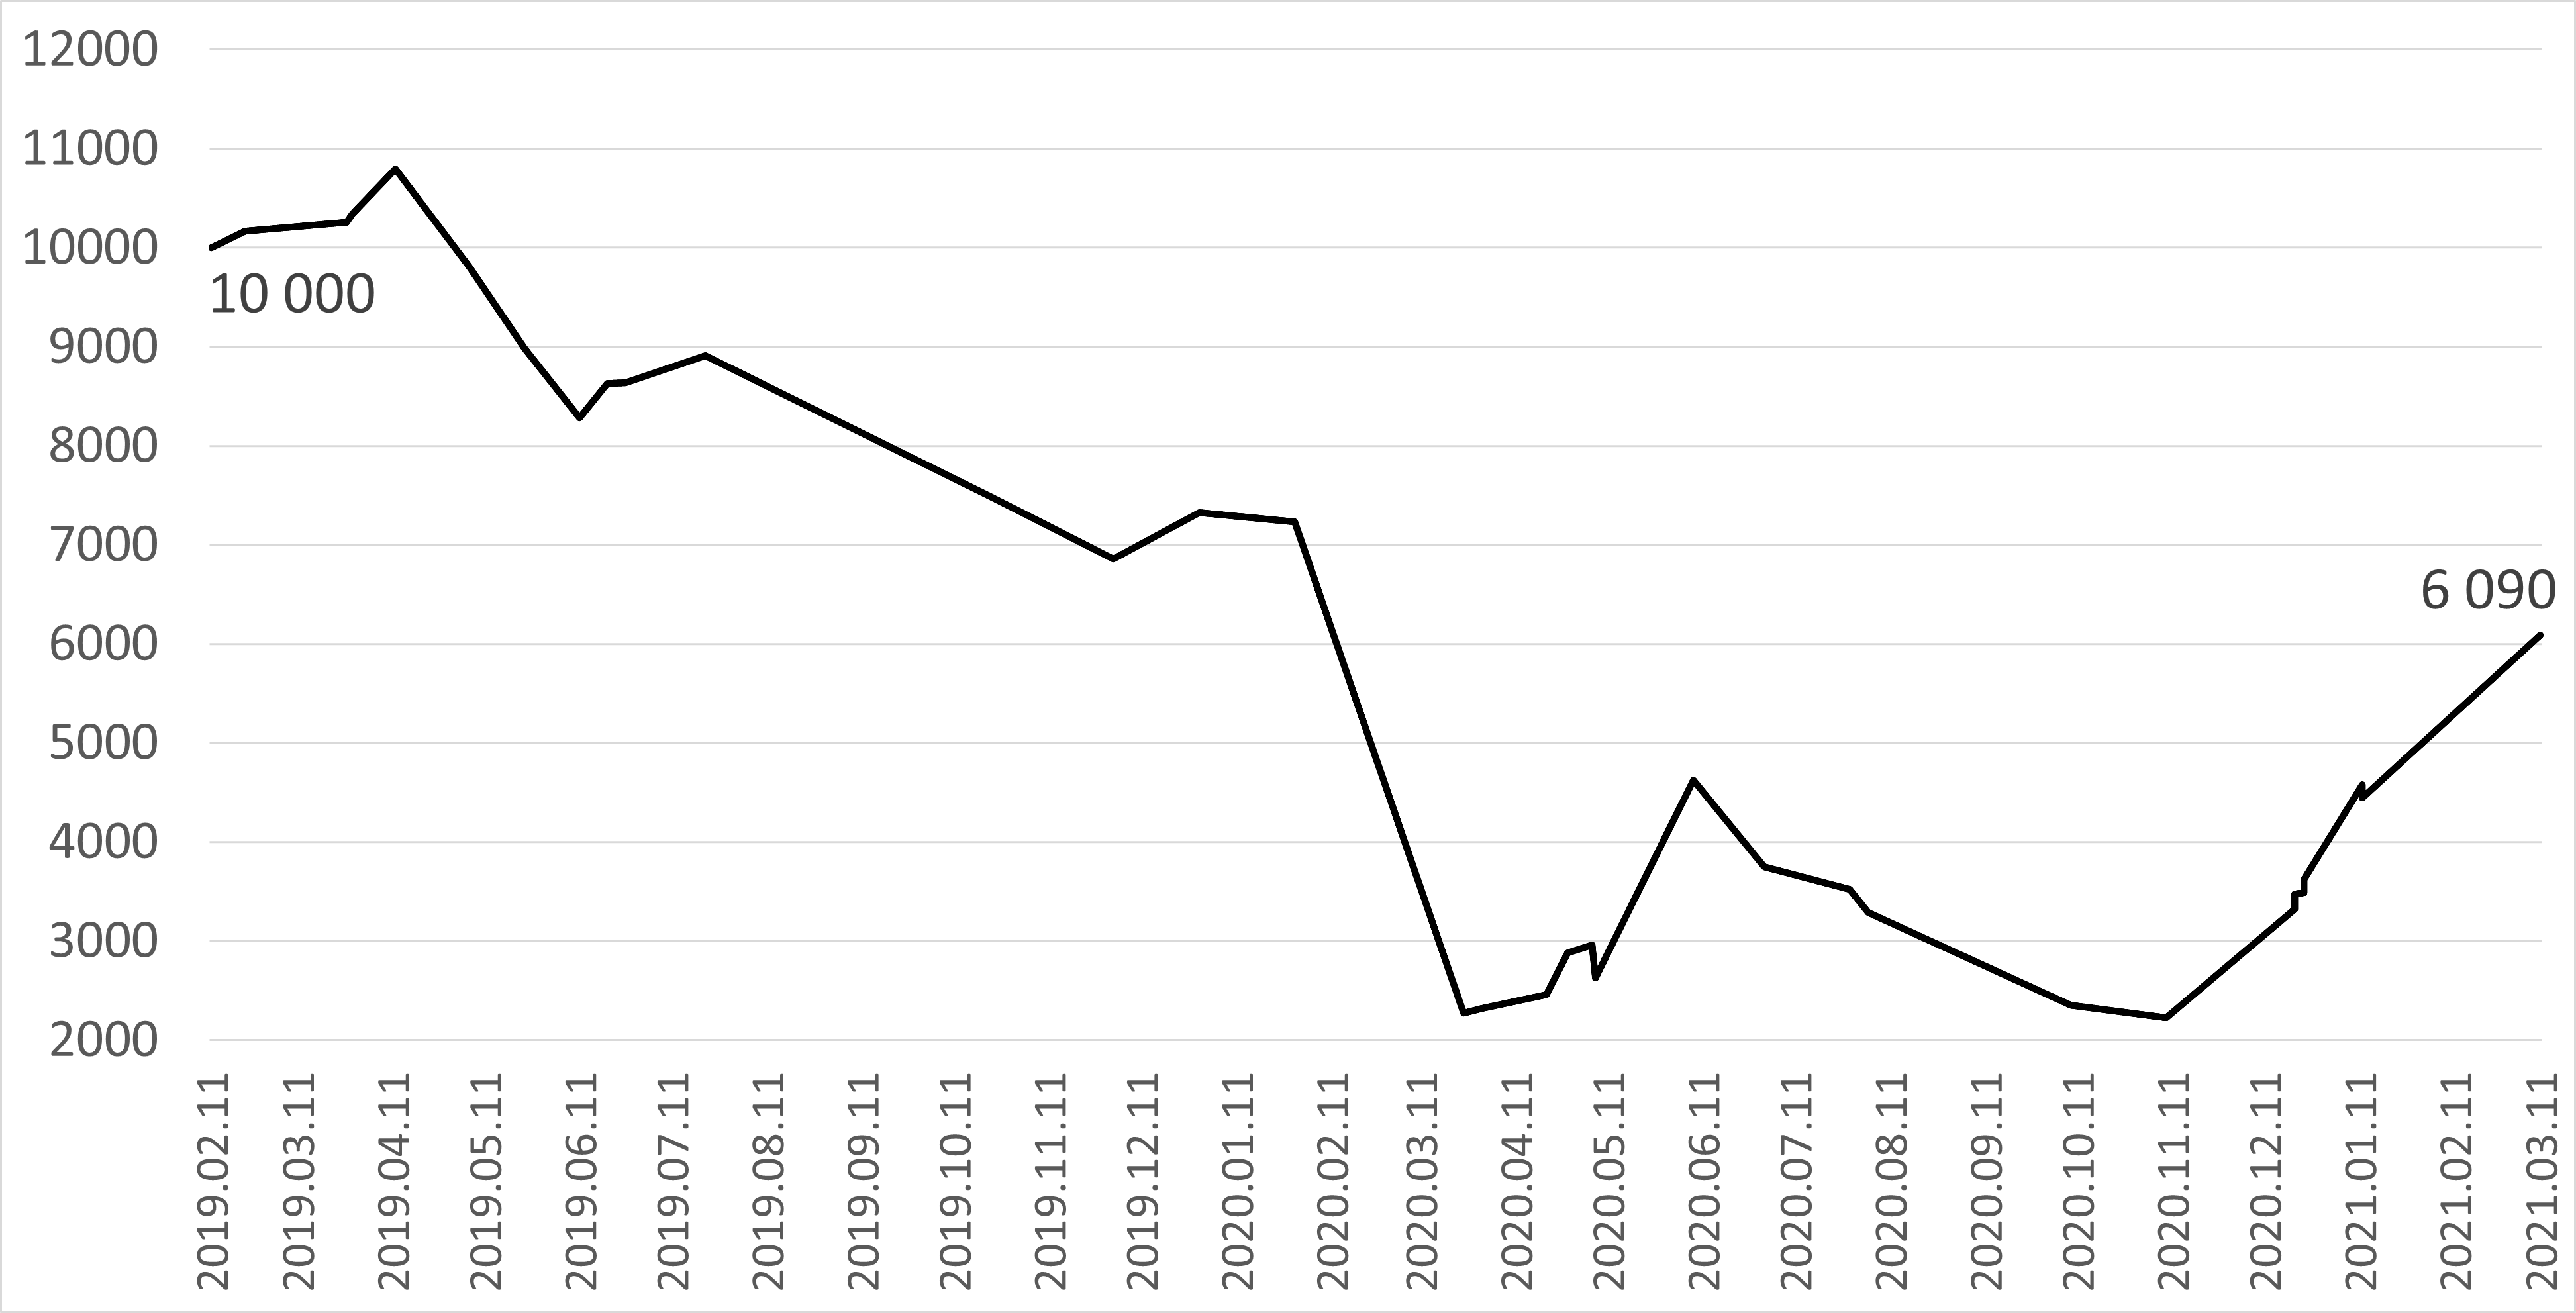
\includegraphics[width=\textwidth]{images/OXY_MONEY.png}
\caption{A tőke ingadozása az OXY részvényén.}
\label{fig:OXY_MONEY}
\end{figure}

Ha megnézzük ezeket a részvényeket, egy közös pontot találhatunk bennük. Március 16-án a részvények nagy része hatalmasat csökkent, miután a világjárvány komollyá vált. 1987-óta nem történt ekkora esés a részvényeknél. Szerencsére sikerült kilábalni a gödörből, azonban látható, hogy az automata profitját is sikerült lecsökkenteni. A következő fejezetben olyan tényezőkről szeretnék szót ejteni, amiket az automata nem tud időben felfedezni, és nem garantált a nyereségessége.
